% fixture: tikz/matrix
% tier: T3
% engine: document
% specials: compare
% covers: \matrix: cells of path commands split at & and \\, each a picture of its own in an alignment, row sep and column sep, the matrix's node drawn
\documentclass{article}
\usepackage{tikz}
\begin{document}
A matrix 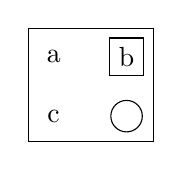
\begin{tikzpicture}
\matrix[draw, column sep=5mm, row sep=3mm] { \node {a}; & \node[draw] {b}; \\ \node {c}; & \draw (0,0) circle (2mm); \\ };
\end{tikzpicture} end.
\end{document}
